\documentclass{article}
\usepackage[utf8]{inputenc}
\usepackage{xcolor}
\usepackage[english]{babel}
\usepackage{graphicx}
\usepackage{listings}
\usepackage{algorithm}
\usepackage{algpseudocode}
\usepackage{arevmath}
\usepackage[hidelinks]{hyperref}
\usepackage{longtable}
\usepackage{multicol}

\definecolor{codegreen}{rgb}{0,0.6,0}
\definecolor{codegray}{rgb}{0.5,0.5,0.5}
\definecolor{backcolour}{rgb}{0.95,0.95,0.92}

\lstdefinestyle{codeStyle} {
    backgroundcolor=\color{backcolour},
    commentstyle=\color{codegreen},
    keywordstyle=\color{blue},
    numberstyle=\tiny\color{codegray},
    stringstyle=\color{magenta},
    basicstyle=\ttfamily\footnotesize,
    breakatwhitespace=false,         
    breaklines=true,                 
    captionpos=b,                    
    keepspaces=true,                 
    numbers=left,                    
    numbersep=5pt,                  
    showspaces=false,                
    showstringspaces=false,
    showtabs=false,                  
    tabsize=2
}
\lstset{style=codeStyle}

\begin{document}

\begin{titlepage}
    \begin{center}
        \vspace*{1cm}
 
        \Huge
        \textbf{Kruskal's Minimum Spanning Tree}
 
        \vspace{0.5cm}
        \LARGE
        CSE 4614 Technical Report Writing
        
 
        \vspace{1.5cm}
 
        \textbf{Shakleen Ishfar}\\
        ID: 160041029
 
        \vspace{2.5cm}
 
        \Large
        Department of Computer Science and Engineering\\
        Islamic University of Technology\\
        Bangladesh\\
        04 August, 2019
 
        \vfill
 
    \end{center}
\end{titlepage}
 
\tableofcontents
\listoffigures
\listoftables

\section{Introduction}
\emph{Kruskal's algorithm} is a \emph{minimum-spanning-tree (MST)} algorithm which finds an edge of the least possible weight that connects any two trees in the forest. The algorithm was written by \emph{Joseph Kruskal} and published in 1956 at the \emph{Proceedings of American Mathematical Society}.

\section{Problem Formulation}
Before getting to the problem statement there are some terminologies which need to be addressed.
\newline
\textbf{Spanning tree: }
A \emph{spanning tree} of a connected and undirected graph is a sub-graph which is a tree connecting all the vertices together. A single graph can have many different spanning trees. The weight of a spanning tree is the sum of weights given to each edge of the spanning tree.
\newline
\textbf{Minimum Spanning Tree: }
A \emph{minimum spanning tree (MST)}, for a weighted, connected and undirected graph, is a spanning tree with weight less than or equal to the weight of every other spanning tree.
\newline
\textbf{Problem Statement: }
Given, a weidghted, connected and undirected graph having V vertices. Kruskal's algorithm will return a graph which will be tree having $V-1$ edges. The total weight of the MST, W is supposed to be equal or less than all other possible spanning trees. Here W is the following:
\begin{equation}
    W = \sum_{i=1}^{V-1}{W_i}
\end{equation} 
where $W_i$ is the weight of the i-th edge of the MST.

\section{General Solution}
Before jumping into the steps of Kruskal's Algorithm some basic knowledge is required to understand the procedure of the algorithm. These are discussed here.

\subsection{Union-Find by Rank}
The union by rank algorithm is used in Kruskal's MST algorithm for cycle detection. A short explanation of Union by Rank is given here for convenience.
\newline
\textbf{Rank: } A rank is basically the maximum depth value of a tree.
\newline
\textbf{Union-Find Algorithm: }
In Union-Find algorithm, a tree having a lower rank is attached to a tree having a higher rank. In other words, the shorter tree is attached to the larger tree. What this algorithm does is that all the vertices in a tree is thought of as being under the same set. Let's say we have a tree with vertices 1, 2, 3 and 4. Then all the vertices of this tree will be seen as being under the same set. Again, let there be two trees respectively having vertices 1, 2, 3 and 4, 5. Then the vertices of each tree will belong to a separate set. Each set is given a value, typically one of the values of the vertices. So a set having 1, 2, 3 might be assigned the value of either 1 or 2 or 3 and the set with members 4, 5 might be given the value of 4 or 5. Now there are essentially 3 operations in this algorithm. 
\begin{enumerate}
    \item \textbf{Union(u, v): } Unites the sets u and v. So merging sets {1, 2, 3} and {4, 5} will result in {1, 2, 3, 4, 5}.
    \item \textbf{FindParent(u): } FInds the parent node of the set u. Meaning, the assigned value for that set.
    \item \textbf{MakeSet(u): } Creates a set with one member u and assigns the set to have u as it's assigned value.
\end{enumerate}

\subsection{Union by Rank in Cycle Detection}
Let's say that initially a vertice will belong to a set that is assigned a value of the vertice value. A group of connected vertices will be under the same set, represented by a value of one of the member vertices (Following the rule of Union-Find algorithm). We shall call this specific vertice as the parent vertice of this group of vertices. Now, when we add a vertice to this graph of connected vertices through an edge we are essentially adding the new vertice set to the group vertice set. Simply, we are merging their set. This is done using Union(u, v) operation. Now, a cycle will form if, we try to add a vertice through an edge that is already in the set of the group of vertice set. So, checking for the set assigned value using FindParent(u) is enough to detect a cycle in the graph. This is how we use the Union-Find by Rank algorithm in Kruskal to detect cycles. There is a much more efficient implementation of Union-Find algorithm that implements path compression to reduce time complexity even more. However, discussion of this implementation is outside the scope of this tutorial.


\subsection{Procedure}
This is a Greedy Algorithm. Here the Greedy Choice is to pick the smallest weight bearing edge that does not form a cycle in the MST constructed so far. The steps to finding the MST of a graph is written below:
\begin{enumerate}
    \item Sort all the edges in non-decreasing order of their weight.
    \item Pick the smallest edge. Check if it forms a cycle with the spanning tree formed so far. If cycle is not formed, include this edge. Else, discard it. Cycle detection is done using \emph{Union by Rank and Path Compression} algorithm.
    \item Repeat step 2 until there are $V-1$ edges in the spanning tree.
\end{enumerate}

\subsection{Kruskal's Algorithm Pseudocode}
\begin{algorithm}
    \caption{Kruskal’s algorithm}
    \label{kruskal}
    \begin{algorithmic}[1]
        \Procedure{Kruskal}{$G$}
        \State $A = \emptyset$
        \Comment Will store MST to be produced
        \For{$v \in G.V$}
        \Comment Each vertice originally in it's own set
            \State \texttt{MakeSet(v)}
            \Comment Makes vertice v a set of v
        \EndFor
        \State \texttt{Sort G.E by non-decreasing weight}
        \Comment Sorts edges of graph G
        \For{$(u, v) \in G.E$}
        \Comment For each edge in graph G
          \If{\texttt{FindSet(u)} $\ne$ \texttt{FindSet(v)}}
          \Comment Check cycle formulation
            \State $A = A \cup {(u, v)}$
            \Comment Add to MST graph
            \State \texttt{Union(FindSet(u), FindSet(v))}
            \Comment Unite u and v parent sets
          \EndIf
        \EndFor
        \State \Return A
      \EndProcedure
    \end{algorithmic}
\end{algorithm}

\section{Example}
To better understand Kruskal's algorithm let us take a look at an example. The example graph is shown in figure \ref{fig:example} We can see that it is a bidirectional weighted graph. So Kruskal's algorithm can be applied to it to find it's MST. Let us simulate the running of the algorithm and see what happens in each step to get a good grasp of how it is working.

\begin{figure}[h!]
    \centering
    \caption{Example graph}
    \label{fig:example}
    \includegraphics{Figures/Complete.jpg}
\end{figure}

The first step is to sort all the edges in non-decreasing order of weight. Any sorting algorithm can be used for this purpose. Sorting the edges yields the following ordering of edges shown in table \ref{table:edgesort}.
\begin{table}[h!]
    \begin{center}
    \caption{Result of sorting edges of example graph}
    \label{table:edgesort}
    \begin{tabular}{|c|c|c|}        \hline
        Weight &  Src  &  Dest  \\  \hline
        1      &   7   &   6    \\  \hline
        2      &   8   &   2    \\  \hline
        2      &   6   &   5    \\  \hline
        4      &   0   &   1    \\  \hline
        4      &   2   &   5    \\  \hline
        6      &   8   &   6    \\  \hline
        7      &   2   &   3    \\  \hline
        7      &   7   &   8    \\  \hline
        8      &   0   &   7    \\  \hline
        8      &   1   &   2    \\  \hline
        9      &   3   &   4    \\  \hline
        10     &   5   &   4    \\  \hline
        11     &   1   &   7    \\  \hline
        14     &   3   &   5    \\  \hline
    \end{tabular}
    \end{center}
\end{table}

Now that our edges have been sorted in non-decreasing order we can begin to include the edges to form our MST. The rule to remember is that we include an edge to our MST only if it doesn't create a cycle. If the edge causes a cycle we will not include that edge. We shall do this as long as we don't have $V-1$ number of edges. Recall V is the number of vertices present in a graph. For our example graph of figure \ref{fig:example} $V = 9$. So we will keep including edges until there are exactly 8 edges in our MST. So let's go through the sorted list and try to formulate our graph one edge at a time, as shown in table \ref{table:steps}.

\begin{longtable}[c]{|p{2cm}|p{2cm}|p{2cm}|p{4cm}|}
    \caption{Going through the graph one edge at a time\label{table:steps}}\\
    
    \hline
    \multicolumn{4}{|c|}{Begin of Table}\\
    \hline
    Edge    & Cycle?  & Verdict & Figure\\
    \hline
    \endfirsthead

    \hline
    \multicolumn{4}{| c |}{Table Continued}\\
    \hline
    Edge    & Cycle?  & Verdict & Figure\\
    \hline
    \endhead
 
    \hline
    \endfoot
    
    \hline
    \multicolumn{4}{| c |}{End of Table}\\
    \hline
    \endlastfoot

    7-6     & No      & Include & 
    \raisebox{-\totalheight}{\includegraphics[width=0.3\textwidth, height=7mm]{Figures/1.jpg}}
    \\  \hline
    8-2     & No      & Include & 
    \raisebox{-\totalheight}{\includegraphics[width=0.3\textwidth, height=30mm]{Figures/2.jpg}}
    \\  \hline
    6-5     & No      & Include & 
    \raisebox{-\totalheight}{\includegraphics[width=0.3\textwidth, height=30mm]{Figures/3.jpg}}
    \\  \hline
    0-1     & No      & Include & 
    \raisebox{-\totalheight}{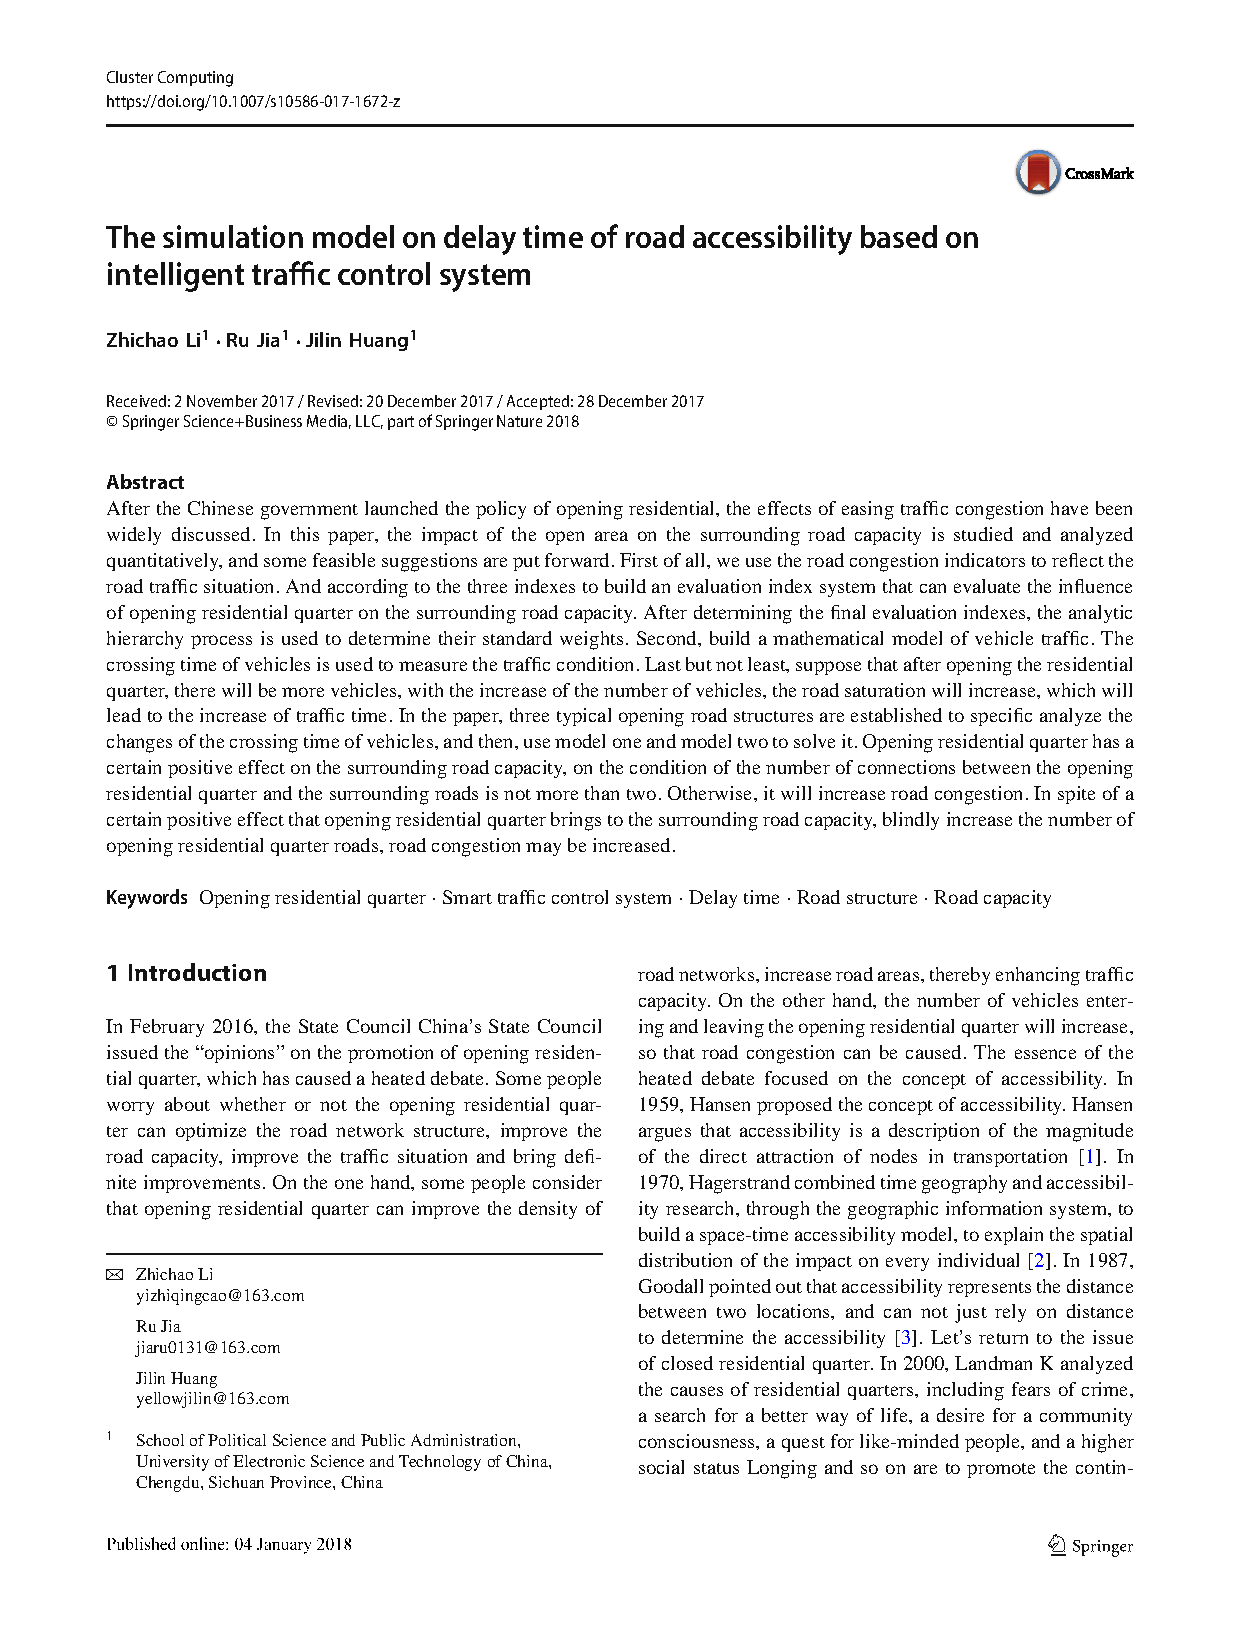
\includegraphics[width=0.3\textwidth, height=30mm]{Figures/4.jpg}}
    \\  \hline
    2-5     & No      & Include & 
    \raisebox{-\totalheight}{\includegraphics[width=0.3\textwidth, height=30mm]{Figures/5.jpg}}
    \\  \hline
    8-6     & Yes     & Discard & 
    \raisebox{-\totalheight}{\includegraphics[width=0.3\textwidth, height=30mm]{Figures/5.jpg}}
    \\  \hline
    2-3     & No      & Include & 
    \raisebox{-\totalheight}{\includegraphics[width=0.3\textwidth, height=30mm]{Figures/6.jpg}}
    \\  \hline
    7-8     & Yes     & Discard & 
    \raisebox{-\totalheight}{\includegraphics[width=0.3\textwidth, height=30mm]{Figures/6.jpg}}
    \\  \hline
    0-7     & No      & Include & 
    \raisebox{-\totalheight}{\includegraphics[width=0.3\textwidth, height=30mm]{Figures/7.jpg}}
    \\  \hline
    1-2     & Yes     & Discard & 
    \raisebox{-\totalheight}{\includegraphics[width=0.3\textwidth, height=30mm]{Figures/7.jpg}}
    \\  \hline
    3-4     & No      & Include & 
    \raisebox{-\totalheight}{\includegraphics[width=0.3\textwidth, height=30mm]{Figures/8.jpeg}}
    \\  \hline
\end{longtable}

The final figure in table \ref{table:steps} is our MST. As we'd already added $V - 1 = 8$ edges, we did not need to go through all the edges in table \ref{table:edgesort}. This is how Kruskal's algorithm can be used to process a graph and build an MST.

\section{Complexity Analysis}
Kruskal's algorithm has a complexity of O(VlogV). We get this complexity in the following way:
\begin{itemize}
    \item To sort the edges in non-decreasing order of weight, we can use merge or quick sort. This takes O(ElogE) time.
    \item We iterate through all edges E and apply find-union algorithm. The find and union operations can take at most O(logV) time.
    \item To perform both these operations complexity becomes O(ElogE + ElogV).
    \item The value of E can be at most O($V^2$), so O(logV) are O(logE) same. Thus, ultimately time complexity becomes O(VlogV).
\end{itemize}


\end{document}
